\markedchapter{Topological states}{Topological states of matter \& symmetries}\label{chap:topo-states}

\blue{Sources: \cites{Akhmerov_online-course}{Asboth_topo-course}{Bernevig_topological-insulators}{Sato_superconductors}}

\blue{Topo phases occur in nature: \cite{Gehring_natural-TI}}

\red{Finish intro when chapter is more complete} %TODO

\section{Basic definitions}
{\color{blue}
\begin{itemize}
	\item Conducting properties of materials are understood in terms of band structure → Fermi energy. Conductance means Fermi level lies inside one of the bands. [picture]
	
	\item $N$-band system has hilbert space $\Hc\cong\C^N$, Hamiltonian represented by $N\times N$ matrix. Static system: $H\psi = E\psi$, eigenvalues are energy bands.
	
	\item Mostly interested in 2-band systems since only valence/conduction bands are relevant. Then $H$ is a $2\times 2$ Hermitian (for now) matrix. These are given by $H = h_0\Id + \h\cdot\bm{\upsigma}$ in general ($h_0$ changes the energy of all bands but does not affect topology of band crossings) → Bloch Hamiltonian [higher dimensional systems: Clifford algebra]
	
	\item For a Bloch Hamiltonian, eigenvalues are $\pm\abs{\h}$, so conductance occurs when $\h = 0$.
	
	\item Insulating Hamiltonians are adiabatically connected if they can be continuously deformed into each other without band crossings. Insulators are considered topological if they are not adiabatically connected to a reference trivial phase; then these inhabit different regions of the phase diagram → existence of edge states (not always \cite{Bernevig_topological-insulators}, footnote)
\end{itemize}
}

\subsection{Bloch theory}
{\color{blue}
\begin{itemize}
	\item We work with crystalline materials which are composed of periodically repeating unit cells.
	
	\item In the bulk, we assume the Hamiltonian is periodic in the unit cell. This enables use of Bloch's theorem \cite{Bloch_theorem} $\psi(\vb{r}) = \e^{i\k\cdot\vb{r}}u_{\k}(\vb{r})$.
	
	\item Different values of crystal momentum may yield identical eigenstates, the set of equivalence classes is the Brillouin zone
	
	\item Brillouin zone usually has $\T^n$ topology, but internal symmetries etc. may alter this \cite{Fonseca-Vaidya_nonorientable} [other sources]
	
	\item Discuss dispersion relations
\end{itemize}
}


\markedsection{The SSH model}{The Su--Schrieffer--Heeger model}\label{sec:SSH}
{\color{blue}
	\begin{itemize}
		\item SSH is usually introduced "physics first", but we would like to work backwards in a sense, to see how bulk topology gives rise to physical properties of a system.
	\end{itemize}
}

We will take the approach of deriving the Su--Schrieffer--Heeger (SSH) model by beginning with a generic one-dimensional crystal, and introducing two topologically distinct phases in the simplest way possible.

Concretely, consider an infinite one-dimensional chain of unit cells indexed by $n\in\Z$; at this point, we make no assumptions on the internal structure of these unit cells. A boundary will be introduced later, but its relevant properties will turn out to be determined by the crystal's bulk topology. Suppose the real-space Hamiltonian of the system is periodic in the unit cells. By Bloch's theorem, two crystal momenta $k$ and $k'$ are then equivalent if they differ by an integer multiple of $2\pi$. This means that the Brillouin zone $B$ can be taken to be the interval $[-\pi,\pi]$, with the points $-\pi$ and $\pi$ identified; this space is homeomorphic to the circle $S^1$.

We might begin with a simple two-band Bloch Hamiltonian $H(k) = \h(k)\cdot\bm{\upsigma}$, with
\[
	\h: B\cong S^1\to\R^3,\quad k\mapsto\begin{pmatrix}
		h_x(k) \\ h_y(k) \\ h_z(k)
	\end{pmatrix}.
\]
Such a Hamiltonian describes a gapped phase precisely when the map $\h$ is non-zero everywhere, so that the topological classification of these phases is given by classes of maps from $S^1$ to $\R^3$ minus the origin---that is, homotopy classes of loops in $\R^3\setminus\set{0}$. However, this space has a trivial fundamental group $\pi_1\big(\R^3\setminus\set{0}\big)\cong0$, meaning that all such loops can be contracted to a point; in other words, all gapped Hamiltonians are adiabatically connected, and there are no topologically interesting phases.

This situation can be remedied by imposing a constraint on the Hamiltonian: we require that $h_z(k)=0$. Doing this effectively reduces $\h$ to a two-dimensional map:
\[
	\h: B\cong S^1\to\R^3,\quad k\mapsto\begin{pmatrix}
		h_x(k) \\ h_y(k)
	\end{pmatrix}.
\]
The gapped phases are now classified by the non-trivial fundamental group $\pi_1\big(\R^2\setminus\set{0}\big)\cong\Z$. This group is indexed by winding number: loops that wind around the origin $a\in\Z$ times cannot be deformed into those with a different winding number $b\neq a$. In particular, loops with a non-zero winding number cannot be contracted to a point, and the associated phases are considered topological. Note that imposing a constraint on the Hamiltonian has made this system rather more interesting from a topological point of view, even though it seems like it has been simplified. Once we move to the physical picture, we will see that this restriction corresponds to imposing a certain symmetry on the system.

Let us now choose a more specific Hamiltonian to arrive at a concrete physical system. We begin with the simplest possible\footnote{
	Our particular choice of $x$, $y$, and $z$ coordinates very conveniently leads to the SSH model. However, mathematically speaking, all similar models are related by a simple change of basis.}
topologically distinct states, one trivial and one topological:
\[
	\h_{\rm triv}(k) = \begin{pmatrix}
		1 \\ 0 \\ 0
	\end{pmatrix},\qquad \h_{\rm top}(k) = \begin{pmatrix}
		\cos(k) \\ \sin(k) \\ 0
	\end{pmatrix}.
\]
To characterise a phase transition between these two states, we consider the linear combination $\h(k) = v\h_{\rm triv}(k) + w\h_{\rm top}(k)$, with $v,w\geq0$. The phase described by the resulting Bloch Hamiltonian is trivial when $v>w$, gapless (i.e.\ conducting) when $v=w$, and topological when $v<w$; see Figure~\ref{fig:phases}.
\begin{figure}[htb!]
	\centering
	\begin{subfigure}{.3\textwidth}
		\centering
		\begin{tikzpicture}
			\begin{axis}[
				axis equal image,
				axis lines=middle,
				axis line style={->},
				xtick={-1,1}, ytick={-1,1},
				xmin=-1.2, xmax=1.2,
				ymin=-1.2, ymax=1.2,
				xlabel=$h_x$, ylabel=$h_y$,
				width=6.5cm,
				]
				\addplot+[mark options={black}] coordinates {(0,0)};
				\addplot [
				samples=100, domain=0:2*pi, color=teal, thick,
				] ( {.3*cos(deg(x)) + .5}, {.3*sin(deg(x))} );
			\end{axis}
		\end{tikzpicture}
		\caption{$v=0.5$, $w=0.3$}
	\end{subfigure}
	\hfil
	\begin{subfigure}{.3\textwidth}
		\centering
		\begin{tikzpicture}
			\begin{axis}[
				axis equal image,
				axis lines=middle,
				axis line style={->},
				xtick={-1,1}, ytick={-1,1},
				xmin=-1.2, xmax=1.2,
				ymin=-1.2, ymax=1.2,
				xlabel=$h_x$, ylabel=$h_y$,
				width=6.5cm,
				]
				\addplot+[mark options={black}] coordinates {(0,0)};
				\addplot [
				samples=100, domain=0:2*pi, color=teal, thick,
				] ( {.4*cos(deg(x)) + 0.4}, {.4*sin(deg(x))} );
			\end{axis}
	\end{tikzpicture}
	\caption{$v=w=0.4$}
	\end{subfigure}
	\hfil
	\begin{subfigure}{.3\textwidth}
		\centering
		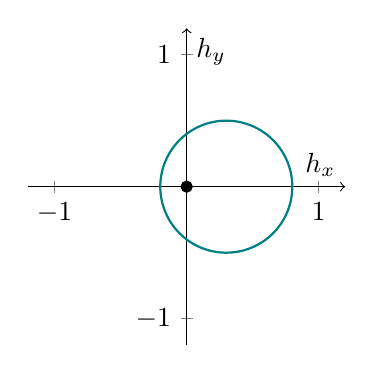
\begin{tikzpicture}
			\begin{axis}[
				axis equal image,
				axis lines=middle,
				axis line style={->},
				xtick={-1,1}, ytick={-1,1},
				xmin=-1.2, xmax=1.2,
				ymin=-1.2, ymax=1.2,
				xlabel=$h_x$, ylabel=$h_y$,
				width=6.5cm,
				]
				\addplot+[mark options={black}] coordinates {(0,0)};
				\addplot [
				samples=100, domain=0:2*pi, color=teal, thick,
				] ( {.5*cos(deg(x)) + 0.3}, {.5*sin(deg(x))} );
			\end{axis}
		\end{tikzpicture}
		\caption{$v=0.3$, $w=0.5$}
	\end{subfigure}
	\caption{Contours in Hamiltonian space for (a) trivial, (b) conducting and (c) topological phases.}
	\label{fig:phases}
\end{figure}

We are now in a position to start analysing the physics of the system. Concretely, the momentum space Hamiltonian is given by
\begin{align*}
	H(k) &= \h(k)\cdot\bm{\upsigma} = \big(v + w\cos(k)\big)\sigma_x + w\sin(k)\sigma_y = \begin{pmatrix}
		0 & v + w\e^{-ik} \\
		v + w\e^{ik} & 0
	\end{pmatrix}.
\end{align*}
We can set up a Fourier transform to real space by rewriting this suggestively in terms of the unit cell index $n$:
\[
	H(k) = \e^{-ik(n-n)}\begin{pmatrix}
		0 & v \\
		v & 0
	\end{pmatrix} + \e^{-ik\big((n+1)-n\big)}\begin{pmatrix}
		0 & w \\
		0 & 0
	\end{pmatrix} + \e^{-ik\big(n-(n+1)\big)}\begin{pmatrix}
		0 & 0 \\
		w & 0
	\end{pmatrix}
\]
{\color{red} I need to work out the details of this Fourier transform later, my calculations aren't working out. Transforming from a periodic Brillouin zone to (discrete or infinite) real space is breaking my brain. I imagine it needs to look something like this (where $M_{0/\pm1}$ are the three matrices above):
\begin{align*}
	\hat{H} &= \int_B H(k) \ket{k}\bra{k} \\
		&= \int_{-\pi}^{\pi}\frac{\dd{k}}{2\pi} \left(\sum_{a\in\{0,\pm1\}}\e^{-ika}M_a\right) \left(\sum_{n}\e^{-ikn}\ket{n}\right) \left(\sum_{n'}\bra{n'}\e^{ikn'}\right) \\
		&= \sum_{a,n,n'}\left(\int_{-\pi}^{\pi}\frac{\dd{k}}{2\pi}\e^{-ik(a+n-n')}\right)M_a\ket{n}\bra{n'} \\
		&= \sum_{a,n,n'}\delta_{n+a,n'}M_a\ket{n}\bra{n'} \\
		&= \sum_{a,n}M_a\ket{n}\bra{n+a}
\end{align*}
But I don't fully understand the first step, the sign of $a$ is wrong and normalization is broken. Maybe it's easier to discretize first and do a DFT?}

{\color{blue}
\begin{itemize}
	\item It follows [how exactly?] that we can write the Hamiltonian in a unit cell basis as
	\[
		\hat{H} = \sum_{n=-\infty}^{\infty}\left[\ket{n}\bra{n}\otimes\begin{pmatrix}
			0 & v \\
			v & 0
		\end{pmatrix} + \left(\ket{n+1}\bra{n}\otimes\begin{pmatrix}
			0 & w \\
			0 & 0
		\end{pmatrix} + {\rm h.c.}\right)\right]
	\]
	
	\item Mention tight binding somewhere around this point
\end{itemize}
}

This Hamiltonian contains a term which acts within the unit cells, and terms which act between neighbouring unit cells, parametrized by $v$ and $w$ respectively. The structure of these interactions can be made somewhat more transparent by going to a finite chain of length $N$. The Hamiltonian then becomes
\[
	\hat{H} = \sum_{n=0}^{N}\ket{n}\bra{n}\otimes\begin{pmatrix}
		0 & v \\
		v & 0
	\end{pmatrix} + \sum_{n=0}^{N-1}\left(\ket{n+1}\bra{n}\otimes\begin{pmatrix}
		0 & w \\
		0 & 0
	\end{pmatrix} + {\rm h.c.}\right),
\]
where open boundary conditions have been introduced on the ends of the chain to allow the boundary behaviour to be studied. The tensor products can be expanded in order to cast the Hamiltonian into a full $2N\times 2N$ matrix:
\[
	\hat{H} = \begin{pNiceMatrix}
		\Block[borders={bottom,right,tikz=dashed}]{2-2}{}
					 0 & v & \Block[borders={bottom,right,tikz=dashed}]{2-2}{}
							 0 & 0 & \Block{4-4}{0} &        &   & \\
					 v & 0 & w & 0 &                &        &   & \\
		\Block[borders={bottom,right,tikz=dashed}]{2-2}{}
					 0 & w & 0 & v &                &        &   & \\
					 0 & 0 & v & 0 &                &        &   & \\
		\Block{4-4}{0} &   &   &   &                & \Ddots & 0 & 0 \\
					   &   &   &   & \Ddots         &        & w & 0 \\
					   &   &   &   &              0 & w      & 0 & v \\
					   &   &   &   &              0 & 0      & v & 0
	\end{pNiceMatrix}.
\]
A physical interpretation of this system presents itself in the form of this matrix: it describes a chain of $2N$ sites, with alternating hopping amplitudes $v$ and $w$ between neighbouring sites. The unit cells now consist of two of these sites, and $v$ and $w$ are referred to as the \emph{intra-cell} and \emph{inter-cell} hoppings, respectively. When these two hoppings are equal, the system is in the gapless phase $v=w$, corresponding to a chain where all bonds are equally strong. Intuitively, this homogeneity allows electrons to propagate freely along the chain. On the other hand, in the insulating cases $v\neq w$, one of the two hoppings is stronger than the other, and the electrons tend to be confined around these stronger bonds.

Dividing the unit cells into two individual sites in this way allows us to distinguish two so-called \emph{sublattices} of the crystal, which we label $A$ and $B$. The notation can then be simplified by labelling quantum states according to the sublattice on which they are localized:
\[
	\ket{n,A} \equiv \ket{n}\otimes\begin{pmatrix}
		1 \\ 0
	\end{pmatrix},\quad \ket{n,B} \equiv \ket{n}\otimes\begin{pmatrix}
		0 \\ 1
	\end{pmatrix}.
\]
In this notation, the Hamiltonian becomes
\begin{equation}\label{eq:ssh-sublattice}
	\hat{H} = \left(\sum_{n=0}^{N}v\ket{n,B}\bra{n,A} + \sum_{n=0}^{N-1}w\ket{n+1,A}\bra{n,B}\right) + {\rm h.c.}
\end{equation}

The tight-binding model of alternating hoppings is precisely the SSH model: it was introduced in 1979 by Wu-Pei Su, John Robert Schrieffer, and Alan J. Heeger to describe polyacetylene (Figure~\ref{fig:polyacetylene}), a polymer chain which features alternating single and double covalent bonds \cites{SSH_model}{SSH_model2}.
\begin{figure}[htb!]
	\centering
	\includegraphics[width=.8\linewidth]{Images/polyacetylene} %TODO svg
	\caption{Structural diagram of polyacetylene. Electrons are transported more readily along the double bonds, which is modelled using a larger hopping parameter.}
	\label{fig:polyacetylene}
\end{figure}
This material displays unexpectedly high conductivity when doped with halogen impurities, and the SSH model affords an explanation for this.

To understand how this metallic behaviour comes about, the differences between the trivial and the topological phase must be examined more closely. The two phases appear to be identical at a first glance: if the unit cell in polyacetylene is chosen in such a way that the stronger double bond represents the intra-cell hopping $v$, then the system is in the trivial phase $v>w$, and if instead the unit cell is centred around a single bond, $v<w$ and the phase is topological. In either case, valence electrons are expected to remain localized around the double bonds, leading to the same insulating bulk behaviour.\footnote{
	The attentive reader might wonder why the conducting $v=w$ phase does not occur naturally in this system. This is a result of the so-called Peierls transition: in a nutshell, introducing a band gap locally lowers the energy of the (filled) valence band and raises that of the (empty) conduction band. This makes it energetically favourable for atoms in the chain to pair up, in a process referred to as dimerisation.}

The difference between the two phases only becomes apparent when the endpoints of the chain are studied. \red{[introduce a figure here]}%TODO
For example, the leftmost atom is not subject to any inter-cell hopping, and it is only connected to the other atom in its unit cell. In the trivial case, this connection is strong and the two atoms share their valence electrons. In the topological phase, on the other hand, the second atom from the left prefers to share electrons with its right-hand neighbour, and the leftmost atom becomes isolated. In the limit where $v$ goes to zero, this isolation becomes complete and the edge sites carry zero-energy eigenstates. In this case, only the second term in the Hamiltonian \eqref{eq:ssh-sublattice} survives, and the edges obey the eigenvalue equations
\begin{align*}
	\hat{H}\ket{1,A} = \hat{H}\ket{N,B} = 0.
\end{align*}
These edge modes can be shown to persist for non-zero $v<w$, in which case they become highly localized and approach zero energy in the $N\to\infty$ limit.\footnote{
	A precise understanding of this is beyond the scope of this review; the interested reader is referred to e.g.\ \cite{Asboth_topo-course}.}
The salient point is that the boundary modes of the topological phase exist inside the energy gap: their energy eigenvalues have a degeneracy at the Fermi level $\varepsilon_F = 0$. \red{[Perhaps include dispersion figure]}
%TODO picture?

Something remarkable has happened: we have started from a topological description of a gapped bulk phase, and the resulting physical effects appear as in-gap zero energy modes on the boundary of the material. As will become apparent looking at other examples, the existence of edge modes at the Fermi level is a fairly\footnote{
	This is not a completely general statement: topological phases with edge modes at energies other than $\varepsilon_F$ have been shown to be theoretically feasible \cite{Freedman_gapped-edge}. For our purposes, it will be sufficient to restrict our attention to edge modes at the Fermi level.}
general feature of topological phases of matter, captured in the so-called \emph{bulk-boundary correspondence}. It can be thought of as being a result of the inability to go continuously from a topological gapped phase to a trivial one in real space; in particular, the outside boundary of an idealised material connects to the vacuum, which is also considered a trivial gapped phase.

{\color{blue}
\begin{itemize}
	\item Discuss physics of polyacetylene (solitons on trivial/topological interface) and experimental observations of solitons + berry phase \cites{Meier_SSH-soliton}{Atala_SSH-Zak}
	
	\item We can now physically interpret the meaning of setting $h_z = 0$: it ensures that hopping only occurs between the two sublattices $A$ and $B$, and not within them (i.e.\ there are only off-diagonal elements in the internal degrees of freedom). If we define the sublattice projection operators
	\[
		\hat{P}_A = \mathbb{I} \otimes \begin{pmatrix}
			1 & 0 \\ 0 & 0
		\end{pmatrix},\quad \hat{P}_B = \mathbb{I} \otimes \begin{pmatrix}
			0 & 0 \\ 0 & 1
		\end{pmatrix}
	\]
	then the Hamiltonian obeys
	\[
		\hat{P}_A\hat{H}\hat{P}_A = \hat{P}_B\hat{H}\hat{P}_B = 0
	\]
	and so since $\hat{P}_A + \hat{P}_B$ is the identity we have
	\begin{align*}
		\hat{H} &= (\hat{P}_A + \hat{P}_B)\hat{H}(\hat{P}_A + \hat{P}_B) \\
			&= \hat{P}_A\hat{H}\hat{P}_B + \hat{P}_B\hat{H}\hat{P}_A \\
			&= (\hat{P}_A - \hat{P}_B)\hat{H}(\hat{P}_B - \hat{P}_A) \\
			&\equiv -\hat{\Gamma}\hat{H}\hat{\Gamma}
	\end{align*}
	with $\hat{\Gamma}\equiv\hat{P}_A - \hat{P}_B$ having the property that $\hat{\Gamma} = \hat{\Gamma}^{-1} = \hat{\Gamma}\dagger$; this is called sublattice symmetry and it also applies to the momentum space Hamiltonian $H(k)$.
	
	\item An immediate consequence of our setup is that the trivial and topological phase become adiabatically connected if we allow for sublattice symmetry breaking ($h_z \neq 0$).
	
	\item Talk more about $\Z$ invariant (next-nearest-neighbour hopping etc.)
\end{itemize}
}

%\subsection{The Kitaev chain}
%
%{\color{blue}
%\begin{itemize}
%	\item Introduce Majorana modes
%	
%	\item Talk about superconductivity
%	
%	\item Discuss $\Z_2$ invariant vs.\ $\Z$ for SSH topologically
%\end{itemize}
%}

\markedsection{Symmetry classes}{Classification of symmetries}\label{sec:symm-classes}

%TODO Keep to minimum

\section{Higher-dimensional models}\label{sec:insulators}

\subsection{The Chern insulator}\label{sec:Chern}

{\color{blue}
\begin{itemize}
	\item The 2nd cohomology group introduced here classifies complex vector bundles over the Brillouin zone. The vector bundle classification point of view is not one we will pursue in detail in this work, but it is in some ways more fundamental than the description in terms of Berry curvature, especially for systems with additional symmetries. This makes it the preferred point of view for precise mathematical classification schemes.
\end{itemize}	
}

\subsection{Quantum spin Hall effect}\label{sec:QSHE}

{\color{blue}
\begin{itemize}
	\item Introduce the $\Z_2$ FKMI invariant in 2D, both in terms of product-of-signs and EBZ integral. (Perhaps mention twisted equivariant cohomology? Not the classical treatment and may not be necessary at this point)
\end{itemize}
}

\subsection{3D strong and weak insulators}\label{sec:3D-Z2}

{\color{blue}
\begin{itemize}
	\item Refer to tenfold way, weak $\Z_2$ topology on T-invariant 2D subsystems and strong 3D $\Z_2$ invariant based both on POS and difference of weak invariants.
\end{itemize}
}